%%%%%%%%%%%%%%%%%%%%%%% file template.tex %%%%%%%%%%%%%%%%%%%%%%%%%
%
% This is a general template file for the LaTeX package SVJour3
% for Springer journals.          Springer Heidelberg 2010/09/16
%
% Copy it to a new file with a new name and use it as the basis
% for your article. Delete % signs as needed.
%
% This template includes a few options for different layouts and
% content for various journals. Please consult a previous issue of
% your journal as needed.
%
%%%%%%%%%%%%%%%%%%%%%%%%%%%%%%%%%%%%%%%%%%%%%%%%%%%%%%%%%%%%%%%%%%%


\RequirePackage{fix-cm}
%
%\documentclass{svjour3}                     % onecolumn (standard format)
%\documentclass[smallcondensed]{svjour3}     % onecolumn (ditto)
%
%\documentclass[smallextended]{svjour3}       % onecolumn (second format)
\documentclass[twocolumn]{svjour3}          % twocolumn
%
\smartqed  % flush right qed marks, e.g. at end of proof
%
\usepackage{graphicx}
\usepackage[english]{babel}
% \usepackage{mathptmx}      % use Times fonts if available on your TeX system
%
% insert here the call for the packages your document requires
%\usepackage{latexsym}
% etc.
%
% please place your own definitions here and don't use \def but
% \newcommand{}{}
%
% Insert the name of "your journal" with
\journalname{Autonomous Robots}
%
\begin{document}

\title{Jderobot open source framework for robotic, computer vision and home automation applications
%\thanks{Grants or other notes
%about the article that should go on the front page should be
%placed here. General acknowledgments should be placed at the end of the article.}
}
%\subtitle{Do you have a subtitle?\\ If so, write it here}

%\titlerunning{Short form of title}        % if too long for running head

\author{Jos\'e M. Ca\~nas \and David Lobato \and Roberto Calvo \and Julio Vega \and Eduardo Perdices \and Francisco Rivas}

%\authorrunning{Short form of author list} % if too long for running head

\institute{F. Author \at
              first address \\
              Tel.: +123-45-678910\\
              Fax: +123-45-678910\\
              \email{fauthor@example.com}           %  \\
%             \emph{Present address:} of F. Author  %  if needed
           \and
           S. Author \at
              second address
}

\date{Received: date / Accepted: date}
% The correct dates will be entered by the editor


\maketitle

\begin{abstract}
For a given robot most of its intelligence lies on its software, the way it coordinates its sensing and actuation capabilities. In the last years several frameworks have appeared that simplify and speed up the development of robot applications. They favor the code reuse and take benefits from modern software engineering techniques. This paper presents the open source robotics framework Jderobot, a distributed and component oriented platform. It uses explicit interfaces among components and ICE as communication middleware. It provides many tools for robot programming like a template for robot control components, visual HFSM creation, etc. Several examples of research and applications done with this framework are also described as experimental validation of it.
\keywords{Robot software \and Programming frameworks \and Code reuse}
% \PACS{PACS code1 \and PACS code2 \and more}
% \subclass{MSC code1 \and MSC code2 \and more}
\end{abstract}

\section{Introduction}
\label{intro}

%software importance
Most of robot intelligence lies on its software. Once the robot sensor and actuator devices are set, the robot behavior is fully caused by its software. There is no universally accepted way of programming robots. There are robots programmed in low level assembler and also in high level languages like C, C++ or Java. 

The importance of good programming practices has increased in the last years and also the interest in the robotics community on this topic. Several special issues of robotics journals (ARS Special Issue on Software Development and Integration in Robotics, 2006) and books on the topic \cite{brugali2007} have been published, specific workshops and tracks have been created inside ICRA and IROS, the Journal of Software Engineering for Robotics (www.joser.org) has appeared that promotes the synergy between Software Engineering and Robotics, and the Technical Committee for Software Engineering for Robotics and Automation inside the IEEE Robotics and Automation Society (TC-SOFT) has been created. Code reuse, to avoid restarting from scratch for every new robot platform, and software integration are key issues in this area. 

%Encapsulating robot capabilities in functions is a slippery issue as behaviors usually don't fit into the functional abstraction where the caller invokes the function and stops it flow of execution until receives the function response or output.

% software requirements in robotics
Compared with other computer science fields the development of robot applications exhibits some specific requirements. First, liveliness and real-time processing: software here has to take decisions with in a fast way, for instance in robot navigation or image processing. Second, robot software has to deal with multiple concurrent sources of activity, and so tends to be multitask. Third, computing power is usually spread along several connected computers, and so the robotic software may be distributed. Fourth, the robotic software typically deals with heterogeneous hardware. New sensor and actuator devices continually appears in the market and this makes maintenance and portability to new robots or devices more complex. Fifth, the robotic software usually includes a Graphical User Interface, mainly for debugging purposes. Sixth, the robotic software should be expansible for incremental addition of new functionality and code reuse. Seventh, the simulators are very useful in robotics software debugging.

% robotic frameworks 
Mobile robot programming has evolved significantly in recent years, and two approaches are currently found. In the classical approch the application programs for simple robots obtain readings from sensors and send commands to actuators by directly calling functions from the drivers provided by the seller. In last years several frameworks (SDKs) have appeared that simplify and speed up the development of robot applications, both from robotic companies and from research centers, both with closed and open source. They favor the portability of applications between different robots and promote code reuse.

First, they offer a simple and more abstract access to sensors and actuators than the operating systems of simple robots. Using the SDK hardware abstraction layer it deals with low level details accessing to sensors and actuators, releasing the robotics programmer from that complexity.
%For example, in a Pioneer with a laser rangefinder, the applications can obtain readings using ARIA or directly through a serial port. Using ARIA, one need only invoke a method and ARIA will take charge of refreshing the variables. Using the operating system directly, the application must request and periodically read the data from the laser through the serial port, and must identify the protocol of the device to compose and analyze the low level messages correctly. The abstract access is also offered for actuators.

Second, the SDK provides a software architecture for robot applications. It offers a particular way to organize code, handling of code complexity when the robot functionality increases. There are many options: calling to library functions, reading shared variables, invoking object methods, sending messages via the network to servers, etc.. Depending on the programming model the robot application can be considered an object collection, a set of modules talking through the network, an iterative process calling to functions, etc.

Third, usually the SDK includes simple libraries, tools and common functionality blocks, such as robust techniques for perception or control, localization, safe local navigation, global navigation, social abilities, map construction, etc. This way SDKs shorten the development time and reduce the programming effort needed to code a robotic application as long as the programmer can build it by reusing the common functionality included in the SDK, keeping herself focused in the specific aspects of her application. The robot manufacturers sell them separately or include them as additional value with their own SDKs. For example, ERSP includes three packages in the basic architecture: one for interaction, one for navigation and another for vision. 

%% \begin{figure*}
%%   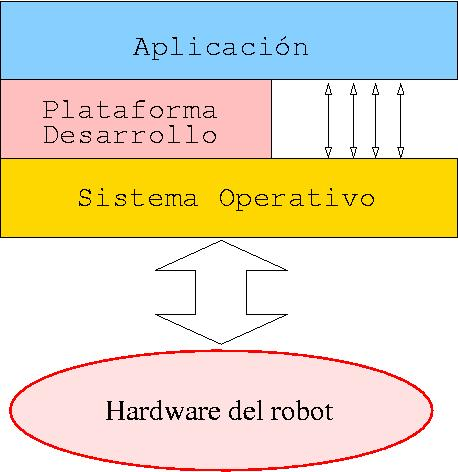
\includegraphics[width=7cm]{figs/programacion3.jpg}
%% \caption{Please write your figure caption here}
%% \label{fig:2}  
%% \end{figure*}

% our proposal
We present our open-source robotic software framework, named Jderobot, which is component oriented, uses ICE as communication middleware and includes several useful tools and libraries. Several sensor and actuator drivers have been programmed or reused from the open-source community. This framework has been widely used in our group for research and teaching for more than ten years. Jderobot has been designed for scenarios with sensors, actuators and intelligent software in between. The typical scenario is robotics, but also computer vision and home automation.

% open source
Why open-source in robotics research? It provides independence on robot manufacturers and so it may support robots from different companies. With the freedom to use and modify the software its final quality does not depend so much on the debugging speed of a single company, distributing the debugging makes it faster. In research, algorithms and results can be replicated and compared. Standard tools (for instance, simulators) and public access to sensor and data repositories (for instance, data bases with input data and ground truth for robot localization), etc. help on this. With this sharing improvements may come more easily and this speeds up the advance as robotics community. In addition, one strong motivation is the feeling of contributing to the community and to return the favor. We have extensively used open-source libraries and tools in our research (OpenCV, Gazebo, GTK, etc.). 

% paper organization
This paper is organized as follows. The state of the art in robotic frameworks fills section \ref{sec:relatedworks}, where other platforms are briefly presented. Section \ref{sec:jderobot} fully explains the proposed platform, the ideas behind its design, the set of standardized interfaces and developed drivers, and the tools included to make the development of new applications easier. In section \ref{sec:applications} some successful examples using Jderobot are presented, both in research and in teaching. Final section summarizes the main conclusions and lessons learnt.

\section{Related works}
\label{sec:relatedworks}

Robotic frameworks can be grouped in two main paradigms, those tightly
coupled with a cognitive model in their designs and those designed
just from a pure engineering criteria. The first ones \textit{force}
the user to follow a set of rules in order to program certain robotic
behavior, while the second ones are just a collection of tools that
can flexibly be put together in several ways to accomplish the task.

%cognitive frameworks
Cognitive robotic frameworks were popular in the 90s and they were
strongly influenced by the AI, where planning was one of the main
keys. Indeed one of the strengths of such frameworks were their
planning modules built around a sensed reality. A good example of cognitive
frameworks was Saphira \cite{konolige98} based on a behavior-based
cognitive model. Some of its low-level functionality was rewritten as a
C++ library called ARIA \cite{aria} that it's still supplied with the
popular robotic platforms from MobileRobots/ActivMedia. Even though
the underliying cognitive model usually is a good practice guide for
programming robots, this hardwired coupling often leads the user to
problems difficult to solve when trying to do something the framework
isn't designed to do.

%current frameworks
Current robotic frameworks focus their designs on the requirements
that robotics applications need and let the user (the programmer) to
choose the organization that better fits with her specific
application. Main requirements driving the designs are: multi-tasking, distributed, easy to
use and code reusability. Another requirement, we believe it's a main
key, it's the open source code, that creates a synergy between the user
and the developer. 

%key achievements
Key achievements of modern frameworks are the hardware abstraction, hiding the complexity of accessing heterogeneous hardware (sensors and
actuators) under standard interfaces, the distributed capabilities
that allow to run complex systems spread over a network of computers,
the multi-platform and multi-language capabilities that enables the
user to run her software in multiple architectures, and the existence
of big communities of software that share code and ideas.

%open source
As said before, we believe that open source plays a major role in the
developement of modern robotic frameworks. Proof of this is the two most popular robotic
frameworks in the last years: Player/Stage
\cite{Gerkey03,collet05,vaughan2007} which has been the \textit{standard de
facto} in most of the last decade and ROS \cite{quigley09} which is
taking the place currently. As seen in other major software projects
as GNU/Linux kernel or the Apache web server, to name but a few, the
creation of communities that interact and share code and ideas, could
be a great benefict to the robotic community. Main examples of open
source modern frameworks are the aformentioned PlayerStage and
ROS. Another important example is ORCA \cite{brooks05,brooks07}. We
briefly describe them.

%%CARMEN \cite{montemerlo03}
There are other open source frameworks that have had some impact on current the state of the art, like RoboComp \cite{bustos2011} by Universidad de Extremadura, CARMEN \cite{montemerlo03} by Carnegie Mellon and Miro \cite{Kraetzschmar02} by University of Ulm. All of them use some component based approach to organize robotic software using ICE, IPC and CORBA, respectively to communicate their modules.

%Non-open source solutions
We can find non open source solutions as well, like Microsoft Robotics Studio or ERSP by Evolution Robotics. 

\subsection{Player/Stage}

Player/Stage framework provides the Player robot device server and the
Stage multiple robot simulator, plus several tools and libraries to support the
development of robotic applications. Player/Stage has been the most
popular framework in the last decade and it has a big community that
has created a great collection of drivers and algorithms around it. It has a platform independent implementation and it has support for the most common programming languages, like C/C++, Python, Java,...

Player provides a network interface to the robot hardware through a collection of standard
interfaces that provides a hardware abstraction layer. These standard interfaces are implemented by drivers, one
for each different hardware. This way a user only needs to know the
standard way to use, let say, a laser ranger and not every different
manufacturer or model. Player exports its devices through a standard TCP network
connection  (other transport layers are available as well)
enabling the user to build distributed systems across a network of
computers. Even though, Player wasn't designed as component based software, its architecture employs many component based
ideas. In addition to hardware drivers, Player has a collection of algorithms
like local navigation algorithms, vision related algorithms or
localization algorithms. 

Stage is a 2.5D multiple robot simulator that can provide its
simulated devices through a Player server. There's a big variety of
devices Stage can simulate, like laser ragers, robotic platforms and
cameras, to name a few.

The typical organization of a robotic application written in Player/Stage is one or more client programms subscribed to a Player server set to serve the robot hardware. Clients send and receive the data using the known interfaces. So, we can say Player/Stage has a centralized architecture, where Player server plays the main role. To run code on the server side, a user can write a driver that implements an interface, but this task it's usually a bit harder that the client side programms and some advanced knowledge of Player/Stage is required.

\subsection{ROS}

ROS is another important example of robotic frameworks. It was founded by Willow Garage as an open source initiative. Currently has a growing community
and its site hosts a great collection of hardware drivers, algorithms
and other tools. It is a multi platform and multi language framework.

Tha main idea behind ROS is a extremely easy to use hybrid (message passing and RPCs) middleware that allows to connect several components, implementing the robotic behavior, in a distributed fashion over a network of computers. Message passing of typed messages allows components to share information in a decoupled way, where you don't know which component send you a message, and viceversa, you don't know which component or components will receive your message. RPC mechanisms are available as well. Resources can be reached through a well defined naming policy.

The ROS core libraries implement the communication mechanisms and a set of tools to help with tasks as project management (cmake based), system
debugging and centralized logging. A set of official libraries implement standard messages (sensors, geometry, action,...), well known robotic algorithms for navigation or sensor analisys, and powerful tools as the \textit{rviz} 3D visualization environment for robots. A simulation enviroment is provided through the Gazebo 3D simulator, that started as a part of the Player/Stage project, but now is supported by Willow Garage.

A typical application written in ROS is a collection of components interacting with each other (no server/client model) distributed among a network of computational nodes. Often a user can just use some of the components found in the ROS repositories, tweak some parameters and make them interact with his own coded components.

\subsection{ORCA}

Another important example is ORCA, a component based framework released several years before ROS. ORCA is multi platform and multi language as well. The aim of its developers was to increase the software reuse among the robotic community, so they create a component repository for robotics applications and they provide some of the needed \textit{glue} to connect them. In a previous version, they coded the middleware that enabled components to communicate. Later they realized that programming a middleware was out of the range of their interests, besides being a complex and time consuming task, so they replaced it with the professional grade middleware Ice from ZeroC \cite{henning04} that allowed them to focus in the robotic problems. ORCA has played a major source of inspiration for the Jderobot framework and some of its core components are closely related to our framework.

As a component based framework, a typical application written in ORCA has an architecture similar to the one described for ROS.

\section{Jderobot platform}
\label{sec:jderobot}
%intro: ya se cuenta en subseccion ``some history''
%The Jderobot platform is the result of the knoledge adquired through
%the development of several projects. The root comes from the doctoral
%thesis \cite{canas02} where the underlying cognitive architecture JDE (acronym in Spanish for Dynamic
%Schema Hierarchy) is
%described. An initial implementation called \textit{jdec} was provided
%where the main idea of organizing the
%software in an intelligent way was developed. Through the years many
%applications have been developed, not only in 
%the robotics field, but in domotic and computer vision fields.

%main characteristics
The Jderobot platform is a component based framework that uses the powerful object oriented middleware Ice from ZeroC as \textit{glue} between its parts. This important design decision allows Jderobot to run in multiple platforms and to be programmed with the most common programming languages (all the languages supported by Ice indeed). Jderobot components can also be distributed over a network of computational nodes and by extension use all the mechanisms provided by Ice as secure communications, redundancy mechanisms or naming services. 

%The platform is supported by a community of developers and its code is open source, released under a GPLv3 licence. A user community is available at \textit{http://jderobot.org}, where users can find documentation, downloads and examples. %%ya se cuenta en seccion jderobot as opensource

%brief description of the underlaying cognitive architecture
The Jderobot platform was developed under the influence of the JDE cognitive architecture \cite{canas02,canas05e}. In early releases, the user was \textit{forced} to follow the main lines of JDE. Currently the underlaying conceptual architecture is just a good practices guide and the user can choose to follow it or not. Briefly, the main lines of the JDE cognitive architecture are as follows:

\begin{itemize}
\item Behavior = {perception} and {control}
\item Divide and conquer: behavior is fragmented is smaller parts called \textit{schemas}
\begin{itemize}
\item[-] Perceptive schemas elaborate estimuli
\item[-] Motor schemas generate control
\end{itemize}
\item A collection of schemas is organized as a dynamic hierarchy
\item Behavior-based aproach
\end{itemize}

The main unit is the schema. A schema is a continous and independent execution flow with some goal. Its activation state can be activated and deactivated at will, and its parameters can be modulated.

%component = schema
The definition of schema has big similarities with the definition of component (from a software engineering point of view), and this is the main link between the Jderobot framework and the underlaying cognitive architecture. A behavior is fragmented in smaller parts (schemas) and then implemented as components.

\subsection{Software architecture design and principles}

The first official public release of Jderobot was 4.3. The core functionality was a collection of shared variables that represented the state of the sensors and actuators attached. A collection of schemas, implemented as a collection of threads, read and wrote these shared variables in order to achieve their goals. There wasn't a explicit API to write or read values from these variables, but just an agreement between writters and readers about the meaning of such variables. Some basic distributed mechanisms where implemented, but mainly as ad-hoc solutions and the main application was centralized on a single machine.

This design worked well for small projects, but as soon as we start implementing more complex systems some important drawbacks arose, like access sincronization, divergencies in the semantics of shared variables among schemas, or the poor distribution solution. All this feedback was very valuable and we chose to completely redesign the Jderobot framework, applying all the lessons learnt.

Following current trends in robotic software engineering we aimed to design a framework with these major requirements:
\begin{itemize}
\item Component based
\item Multi-platform and multi-language support
\item Distributed
\item Strongly typed interfaces
\item Open source
\end{itemize}

%why Ice
Systems with some of these requirements are often hard to build. Because of this, we decided to find an existing middleware that could cope with our requirements. The selection of Ice as the middleware for Jderobot was the most important design decision. This way we could use more efforts to design and program robotic related software and less to deal with problems already solved by Ice where we are no experts. Ice is the main building block of Jderobot.

%component based
The programming model is based on components. A typical Jderobot application is a set of components running concurrently, as different operating system processes. They communicate sharing messages between them, cooperating to achive the desired behavior. Components are the basic unit in Jderobot. A Jderobot component is usually implemented around the \textit{Ice::Application} class running on the main thread of a process, and optionally other service threads performing optional tasks. This main thread execute the component main task, that usually has the form of an iterative task running continously at a specific rate. This iterative task includes the communications task, that sends or receive data. This model is opposed to the one used in previous releases of Jderobot, where basic units were implemented using threads. It's straightforward to see that the use of processes as the basic unit will make easier the approact to the remaining design requirements.

%multi-platform & multi-language
Jderobot is able to interoperate between multiple platforms (Windows, GNU/Linux, MacOS, Android, ...) and it has support for multiple programming languages (C++,Python, Java, PHP,...), as Ice has support for main architectures and for most popular programming languages.

%distributed
Ice provides several communication mechanisms, from syncronous and asyncronous standard RPCs to subscription mechanisms, where multiple publishers and subscribers can interact. This allows Jderobot to provide a rich set of options to provide communication between its components, allowing those components to be distributed over a network of computers. Moreover, Ice has several tools that allows to provide redundant and/or failsafe services.

%interfaces
Jderobot components communicate through interfaces. They define the minimum communication unit between components. Jderobot components implement these interfaces to provide functionality and use them to use the functionality from other components. Interfaces are defined with \textit{slice}, the interface definition language used by Ice, that describe their data structures and operations. These slice definitions are then used to generate code for the desired programming languages.

%open source & software reuse
One development policy in Jderobot is to use open source libraries as much as possible. In addition to Ice, Jderobot uses OpenCV, GStreamer, OpenGL, PCL, Player/Stage or GSL, to name but a few, for the same reasons exposed above: we want to focus our efforts to design and program robotic related software. 
%In return, we release all our code as open source and we encourage our community to follow these ideas.

%gui & config files
Other two minor principles were present in the design process. First, Graphical user interfaces are especially useful for debugging purpouses or for human interaction. Previous releases of Jderobot needed ad-hoc approches because of the multi-threaded design, some wrappers where needed to make the shared access to the screen easier. Nowadays, Jderobot doesn't make any special assumption on this subject, each component is a separate process, the user must choose the approach that better fits in each context. Some guidelines and examples are provided though, through design patterns as MVC or implementations using popular graphic frameworks as GTK+. A Jderobot component usually will run a service thread with the graphical user interface computations. 

Second, components are parameterized and their implementation counterparts require any means to get these parameters. A simple approach is to use configuration files. Ice has native support for parsing simple text files with a format closely related to Java property files. Using this files components can get their specific parameters or the location of resources (files, other components,...). In addition, Ice provides a parameter server that could be used as a central configuration repository.

\subsection{Interfaces and drivers}
\label{sec:drivers}

Beyond previous design principles, the Jderobot framework includes several components that manage different sensors and actuators and provide the applications with standard interfaces for accessing to those devices. Using ICE the access can be local or remote from a different computer. There is no one-to-one relationship between components and interfaces. One driver component may offer several interfaces at the same time, and the same interface may be implemented by several drivers.

% interfaces
There are interfaces for laser devices like Hokuyo, Sick, etc. (\texttt{laser}), for Pioneer base control (\texttt{motors}), for RGB-Depth sensors like kinect, pantilt units (\texttt{pose3Dmotors}, \texttt{pose3Dencoders}), for image sources (\texttt{camera}), for odometry (\texttt{encoders}), for sonar sensors (\texttt{sonars}), for home automation devices (\texttt{x10}), etc.. These interfaces together draw a Hardware Abstraction Layer to be used from the application code. 

Some interfaces are intended to be generic and are offered for different robots, favoring the applications portability. For instance, the \texttt{motors} interface includes translation velocity (V), rotation velocity (W) and side velocity (L). It is supported both by the driver used with the legged Nao robot and by the driver used with the Pioneer wheeled robot (which will ignore the side velocity as not physically plausible on this platform).

The same interfaces are also provided by drivers connected to the real devices and drivers connected to simulators like Gazebo, allowing the applications to run without any modification on the real robot than on simulator. 

% driver component
%PlayerServer, GazeboServer for Gazebo Simulator , NaoServer, KinectServer, OpenNIServer, giraffeServer, PTU, Hokuyo, Wiimote, CameraServer.

\subsubsection{CameraServer}

\texttt{CameraServer} is a component included with Jderobot that serves images from several sources. The underlaying access to images is performed through GStreamer pipelines, and so \texttt{CameraServer} supports all the devices supported by GStreamer, e.g  usb cameras, v4l2 cameras, video files, IP cameras, video streaming or static images. In addition to that, \texttt{CameraServer} offers its resources through RPCs and subscription services.

\subsubsection{PlayerServer}

Jderobot uses Player to access the Pioneer robot sensors and actuators (laser, odometry, motors, etc.). A \texttt{PlayerServer} component wraps the Player software and provides respective ICE standard interfaces. It works both for the real robot or the robot inside the Stage simulator.

\subsubsection{GazeboServer}
\label{subsec:gazeboserver}

Gazebo is the preferred simulator in Jderobot framework. As previously presented, it is a 3D open source simulator (http://gazebosim.org) which offers a rich environment to quickly test multirobot systems and which simulates several robots and cameras in a realistic way.
% It was born inside the Player/Stage/Gazebo project and recently WillowGarage centralized its development as an auxiliar tool for ROS. 
Jderobot includes \texttt{GazeboServer} to communicate applications with devices and robots in Gazebo simulator (\cite{koening2004}). Wrapping the original \texttt{libgazebo} library it's possible to retrieve information from several sensor devices like: laser, encoders, motors, cameras or sonars. It also supports one or more cameras with their corresponding pantilt units (SonyVid30 model).

\begin{figure}[h!]
  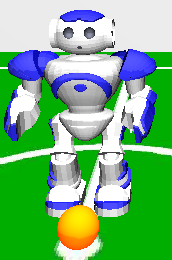
\includegraphics[width=4cm]{figs/nao_piel.png}
  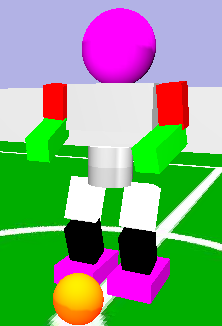
\includegraphics[width=4cm]{figs/nao_sinPiel.png}
\caption{Developed Nao support for Gazebo.}
\label{fig:naogazebo}
\end{figure}

The work in \texttt{GazeboServer} has been extended to simulate the Nao humanoid robot inside Gazebo (Figure \ref{fig:naogazebo} and offer access to its devices through standard ICE interfaces like \texttt{camera}, \texttt{pose3Dmotors} for its neck, \texttt{motors} for its general movement, etc.

\subsubsection{NaoServer}

Nao humanoid robots, from Aldebaran, include the manufacturer's framework called Naoqi, which provides an API to command and read the robot's motors and sensors at different abstraction levels. This API can't be directly deployed by other Jderobot components, since its functions are ad-hoc designed to Nao robots. We have created a component named \texttt{NaoServer}, that runs inside the Nao robots and provides several standard ICE interfaces which may be used by other Jderobot components. NaoServer receives through ICE interfaces commands from other components and translates these commands to Naoqi.

\subsubsection{KinectServer and openniServer}

Kinect is one latest generation devices since it appeared in late 2010. It measures distance to obstacles in 3D using infrared technology. Jderobot includes two drivers, \texttt{kinectServer} and \texttt{openniServer}, to allow access to all the information it provides. Through them applications can access to color, depth and IR values, and also to the tilt motor device and it leds. They provide RGB and depth images as conventional \texttt{camera} interfaces, so these sensors can be used with any Jderobot application following such standard interface.

Both servers use the OpenNi driver developed by PrimeSense. OpenNi is a framework aimed to develop applications that use natural interaction by offering access to low-level devices and also middleware functions for visual tracking using computer vision. \texttt{KinectServer} accesses to the device through the openni\_grabber that PCL includes. This grabber is a very simplified version of the PrimeSense framework and only supports the RGB camera and depth sensor. The \texttt{openniServer} directly uses the OpenNi framework. This driver supports all the kinect components (tilt motor, leds, RGB/IR camera and depth sensor) and offers all the functionality of the middleware. That includes people detection and tracking, user position, hands tracking... Although the servers access information in a different way, both offer information using the same ICE interfaces so both components are completely compatible. 

\subsubsection{X10Server}

A driver inside Jderobot has been developed to support X10 home automation sensors and actuators like lamp modules, occupancy motion detectors, etc.. It uses the \textit{HEYU} open source software. 

\subsubsection{WiimoteServer}

The \textit{Wii} remote from Sony is also supported in Jderobot, with a driver \texttt{wiimoteServer} that provides its accelerometer data, buttons state, its IR data from the local onboard small camera and the state of the \textit{nunchuk} gadget. It uses the \textit{cwiid} open source software.

\subsubsection{Pantilt units}

Two driver components have been developed to provide support for different Pantilt units, one for Directed Perception (PTU-46-17.5) and another for a hand-made one. They provide two interfaces \texttt{pose3Dmotors} to command position movement orders and \texttt{pose3Dencoders} to read the unit pan and tilt position from its internal encoders.

\subsection{Tools and libraries}
\label{sec:tools}

\subsubsection{FuzzyLib}

Fuzzylib is a library to design and program fuzzy controllers. The control rules are written in a file with simple rules like:\texttt{ IF ( left\_obstacle\_distance = small ) AND ( translation\_speed = high ) THEN ( rotation\_speed = right\_high )}. 
%AND and OR fuzzy operators are supported in rules. 
The fuzzy labels and variables are also described in such file following a trapezoidal pattern and they are linked in the software to input and output variables of the control program. The controller automatically fuzzyfies the input variables, apply the rules and defuzzifies the output following a Center of Mass combination.

\subsubsection{VisionLib}
\label{subsec:visionlib}

% It has since been expanded to provide a range of software infrastructure for computer vision, geometry models and images mechanisms. 
This library builds on top of the OpenCV Computer Vision Library\footnote{http://opencv.willowgarage.com/wiki} and the GNU Scientific Library\footnote{http://www.gnu.org/software/gsl} (GSL). It provides some mathematical functions used on visual perception purposes:

\begin{itemize} 
\item \textit{Cvfast} class provides the functionality of the FAST Image Corner Detector with small adaptations.
\item \textit{Geometry} class contains functions for intersections, distances, vector operations, segments operations, etc..
\item \textit{Image} class includes operations such as: Multiply Fast Fourier Transform or Get Segments.
\item \textit{LinesDetection} class provides a Line Detector based on Solis algorithm \cite{solis09}.
%\item \textit{Structs.h} header contains different useful structs for computer vision purposes.
\end{itemize}

\subsubsection{Progeo}
\label{subsec:progeo}

This Projective Geometry library helps in the use of pin-hole calibrated cameras (Figure \ref{fig:pinholemodel}), the relationships between the pixels and the points in 3D space. Some of the data types provided are: \textit{HPoint2D} to store a 2D point that usually belongs to the image plane, \textit{HPoint3D} to represent a point in the 3D space in homogeneous coordinates, and \textit{TPinholeCamera} to store the camera model defined by its extrinsics and intrinsics parameters. It provides the \textit{project} function to project a 3D point on to the 2D image plane, and the \textit{backproject} function to obtain the 3D ray with all 3D points that project in a given pixel inside the image plane.

\begin{figure}[h!]
  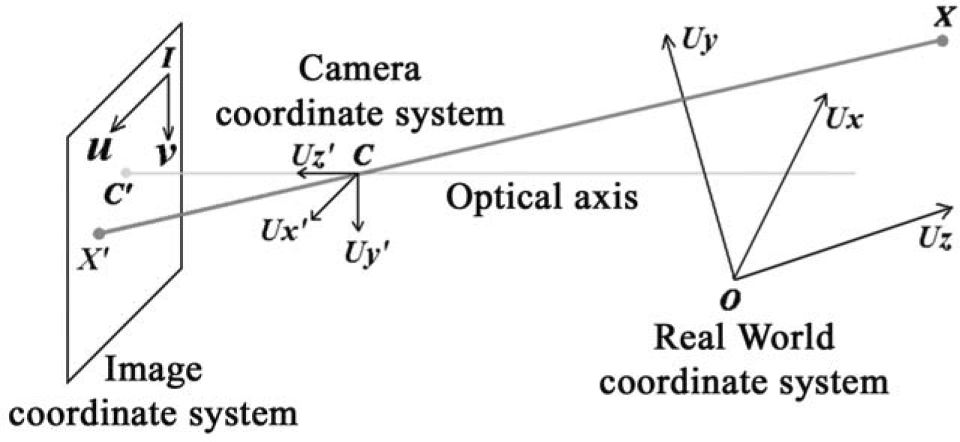
\includegraphics[width=8.5cm]{figs/pinholemodel.png}
\caption{Pin-hole model of a camera.}
\label{fig:pinholemodel}
\end{figure}


\subsubsection{Colorspaces}
\label{subsec:colorspaces}
Colorspaces is a library that provides several routines to handle color space transformations. It has a C implementation for several trasforms that was implemented before OpenCV became mainstream. After adopting OpenCV as the main library to handle images, a C++ implementation was developed. It has a wrapper class for \textit{cv::Image} that can handle color spaces transformations in a transparent way for the user. It is one of the main utility libraries used by Jderobot project.

\subsubsection{Control template}

A \texttt{BasicComponent} is included in Jderobot as a template for reactive controllers. It has two different threads, one for computation and a second one for visualization. Both threads run in continuous iterations at a given configurable rate, not more to avoid excessive CPU consumption. In case of heavy computations or overload of the CPU the system degrades gracefully running at the highest rate possible. This basic component has also been used for perceptive, localization and image processing algorithms.

\subsubsection{VisualHFSM}

There are many ways to organize the control and perception code on board a mobile robot. One succesful way are the Finite State Machines. With them the robot behavior is defined by a set of states, each of which performs a particular task. The robot can switch from one state to another through transitions (conditions of stay or change), depending on certain events or conditions, internal or external. A tool has been developed and included in Jderobot to graphically design hierarchies of FSM, insert the specific code of states and transitions, and automatically generate the component source code in C++.

\begin{figure}[h!]
  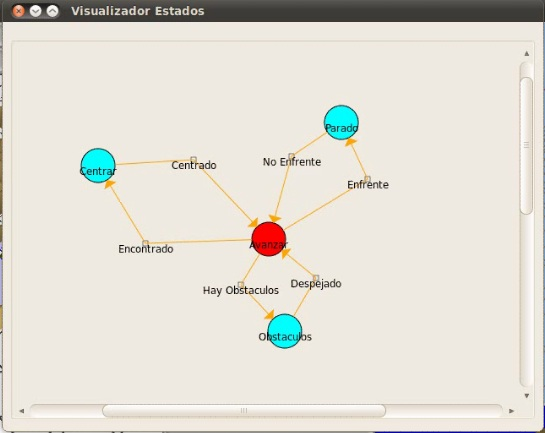
\includegraphics[width=8.5cm]{figs/ratonGatoAutoEjec.jpg}
\caption{Tool for visual HFSM design}
\label{fig:visualHFSM}
\end{figure}

\subsubsection{Calibrator}

The calibrator tool is used to calibrate external (position and orientation) and internal parameters (focal distance, optical center...) of any camera. It allows a manual calibration where the user provides a 3D description of the camera surroundings, the calibrator draws what the image should be with a certain parameter set over the really observed image. The user then modify parameters until finds a correct matching (Figure \ref{fig:calibrator}). It also includes a fully automatic calibration based on DLT and a 3D pattern. It generates a file with the camera calibration parameter values and it is fully integrated with Progeo library.

\begin{figure}[h!]
  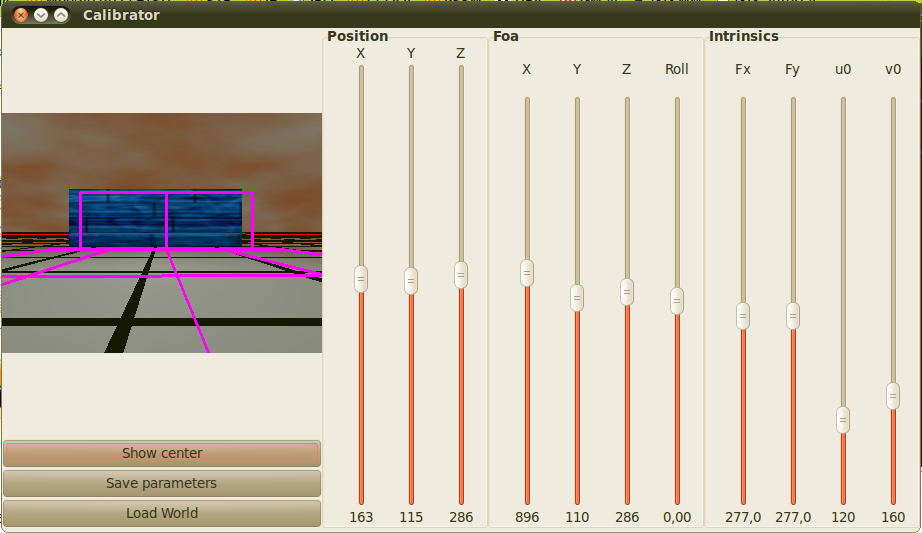
\includegraphics[width=8.5cm]{figs/calibratorGUI.png}
\caption{Calibrator in manual mode}
\label{fig:calibrator}
\end{figure}

\subsubsection{ColorTuner}

The colorTuner tool is used to adjust color filters in different colorspaces, like HSV, YUV, RGB, etc. For instance, the HS color disc is shown (Figure \ref{fig:colortuner}) and the current color filter thresholds are also displayed as a sector. They can be easily modified there, using sliders or clicking in sample pixels in current image.

\begin{figure}[h!]
  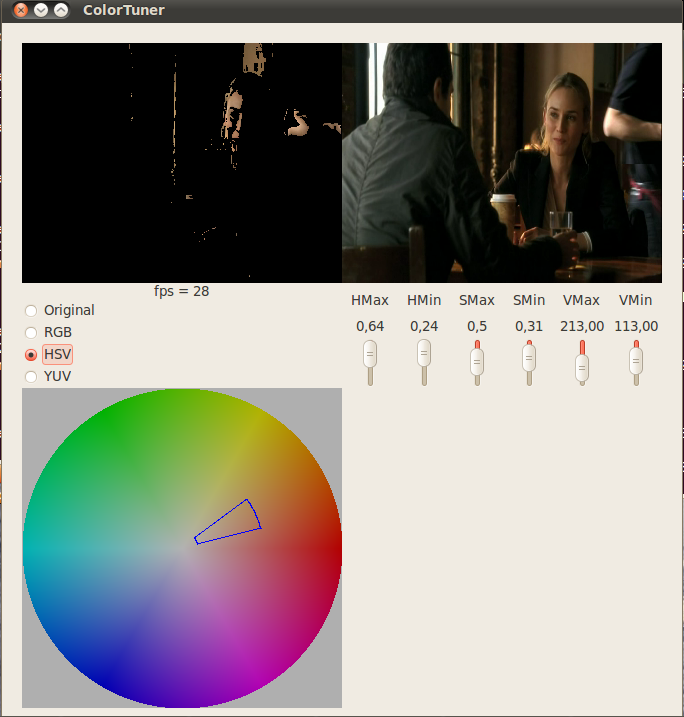
\includegraphics[width=8.5cm]{figs/colorTunerHSV.png}
\caption{ColorTuner tool for adjusting HSV color filters}
\label{fig:colortuner}
\end{figure}


\subsubsection{Recorder and replayer}

When we use real robots, one of the greatest difficulties is repeating experiments with the same conditions, whether we want to compare different algorithms or to test several features of the same algorithm. It's almost impossible to reproduce the same environment conditions, since robot hardware behaves diversely, light conditions change if we use cameras, people or objects move or are located in different places, etc.

To avoid all these matters, we have designed two tools which record the current sensor readings and reproduce them whenever we want to. The first one is the \texttt{recorder} component, it periodically saves in a file the status of all the devices of the robot, such as odometry readings, laser measurements, images from cameras, etc. It is generic, when we execute this tool we can configure which devices we want to track, at which frequency we want to sample the sensor data, etc. It works with simulators, kinect devices, cameras, real Nao robots and real Pioneer robots. The log file includes timestamps and follows a given syntax that is expansible to new sensor types.

The second component is \texttt{replayer} server, it reads the file saved by the \texttt{recorder} component and provides the same ICE interfaces that the drivers with real devices do. Thus, when an algorithm gets the current devices readings, it can't tell if it's obtained in live from the real devices or from pre-recorded data. These two tools have been widely used to perform experiments with real robots, to try different parameters and improve our algorithms.

\subsubsection{Android mobileTeleoperator}

Android operating system is increasing its market share every day, both with smartphones and tablets. 
%Once you develop an application for this platform, it may be used by students, other researchers or even companies. 
We have created an application called \texttt{MobileTeleoperator} to teleoperate either a Pioneer robot through \texttt{playerserver} or a Nao Robot through the \texttt{NaoServer} (Figure \ref{fig:nao-teleoperator}. Connection between the mobile device and the robots is made through ICE, the same way we do when we use a standard computer, so we don't need to change anything in Jderobot architecture.

\begin{figure}[h!]
  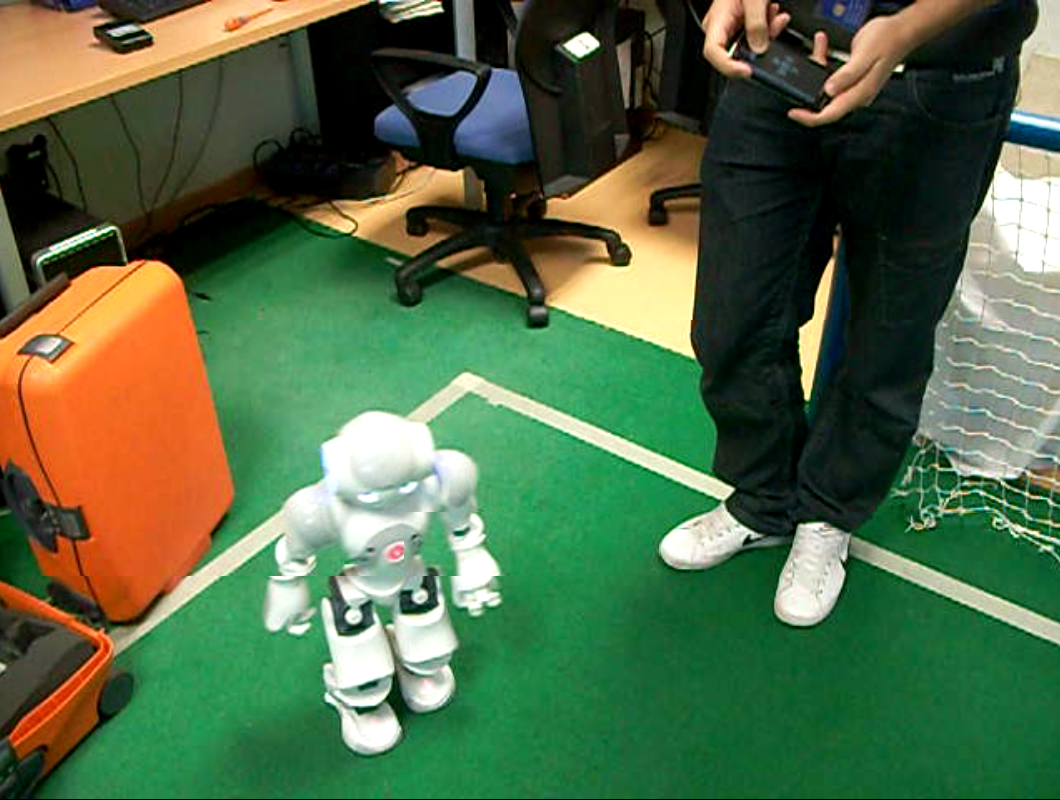
\includegraphics[width=8.5cm]{figs/teleoperator-nao.png}
\caption{Nao robot teleoperated from a smartphone}
\label{fig:nao-teleoperator}
\end{figure}

There are three ways to teleoperate the robots:
- Arrows: After pressing a button, it sends the command to the robot and the robot keeps his behavior until the stop button is pressed.
- Joystick: While a button is pressed, it send the command to the robot, but if the button is released it sends a stop command automatically.
- Accelerometer: It uses the mobile accelerometers to command the robot depending on our device orientation. To use this behavior you must keep a ''safety'' button pressed, this button is used to calibrate the accelerometers when it is pressed the first time and to send a stop command automatically once this button is released.

\texttt{MobileTeleoperator} has been used in exhibitions and to let people not familiar with robot control to teleoperate thema in a easy way.

\subsubsection{KinectViewer}

\texttt{KinectViewer} component is able to connect to one of the kinect servers described in section \ref{sec:drivers}. Basically is a graphical interface witch represents the kinect information in two different ways: it can display directly the images (RGB and DEPTH) that it gets on streaming from the server or it can reconstruct a 3D scene from the point cloud in an OpenGL world. 
%This component also includes some of the 3D tools that jderobot provides to improve the data analysis. 

To work with the cloud of points obtained from the kinect depth sensor Jderobot uses Point Cloud Library (PCL). This library includes a large number of features for point cloud processing such as filters, model fitting and segmentation. 

\section{Research, teaching and applications}
\label{sec:applications}

Once the main software components and design principles of Jderobot have been presented in previous section, in this one we describe some of the succesful research and applications done with it, that somehow probe its usefullness. Applications with sensors and actuators.

\subsection{Teaching robotics with Jderobot}

A component named \texttt{Introrob} has been developed for students to simplify the development of robot control applications in their practices inside several robotics courses at Universidad Rey Juan Carlos. It connects to the Gazebo simulator using \texttt{GazeboServer}, where a Pioneer robot is ready inside a given 3D scenario. Having an integrated simulator is very important, so the students may quickly test their experiments without the need of a robot for everyone. \texttt{Introrob} wraps the ICE interface access and provides a very simple local API with functions to get the sensor readings and set the motor commands. \texttt{Introrob} also shows a GUI with the images from the stereo pair (Figure \ref{fig:introrob}), the laser measurements and a 3D visualization of the scene around the robot. 

\begin{figure}[h!]
  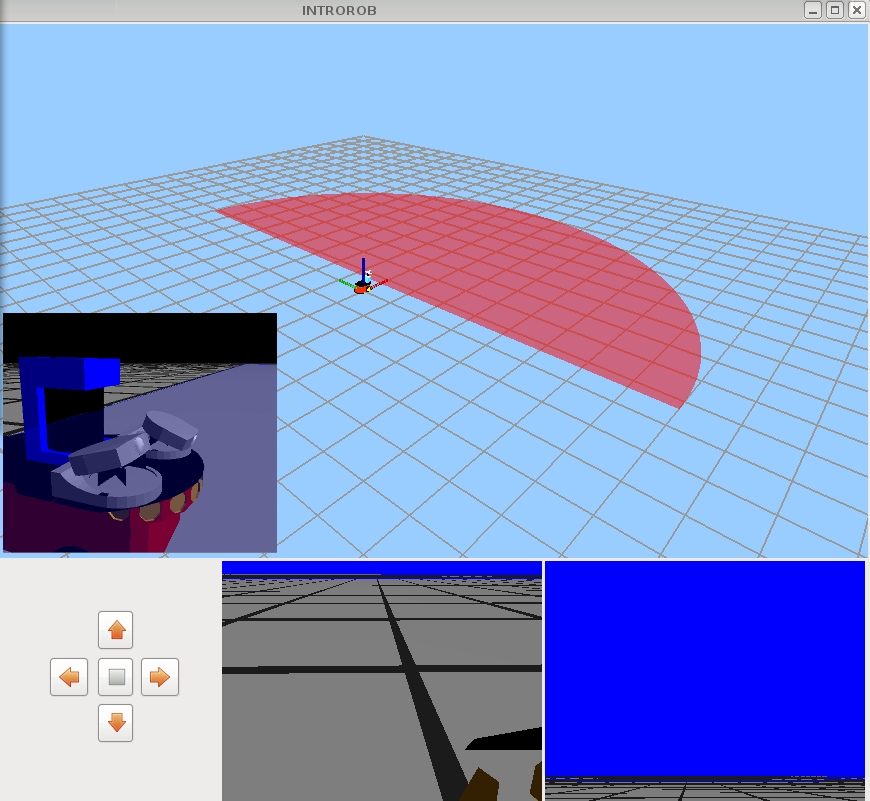
\includegraphics[width=8.5cm]{figs/introrob.jpg}
\caption{Introrob component Graphical interface.}
\label{fig:introrob}
\end{figure}

The processing is organized as in the \texttt{BasicComponent}, with a control thread running iterations periodically (once every 100ms). Students are required to embbed their control software in such iteration code, calling the needed API functions. This way most of the complexity of using Jderobot is hidden and there is no need to know much about gears, motors, sensors, calibration, etc.. This allows students to have a working robot within little over an hour. 

Some of the practices done with this framework are: visual control of a robot following a red line in the floor using a single camera, 3D reconstruction using a stereo pair, local navigation using Virtual Force Field and a cat robot pursuing a mouse (teleoperated) robot using only vision as main sensor.

\subsection{Robot navigation research}

Obstacle avoidance is one of the key issues to successful applications of mobile robot systems. It combines the need of circumventing obstacles and the need to proceed towards the navigation target. We developed an hybrid navigation algorithm that combines two approaches: Virtual Force Field (VFF) as local path planning mechanism, and Gradient Path Planning (GPP) for global navigation. The VFF allows for fast, continuous, and smooth motion of the controlled vehicle among unexpected obstacles. We improved it and adapted to search, track and follow people using vision \cite{canas05d}. 

\begin{figure}[h!]
  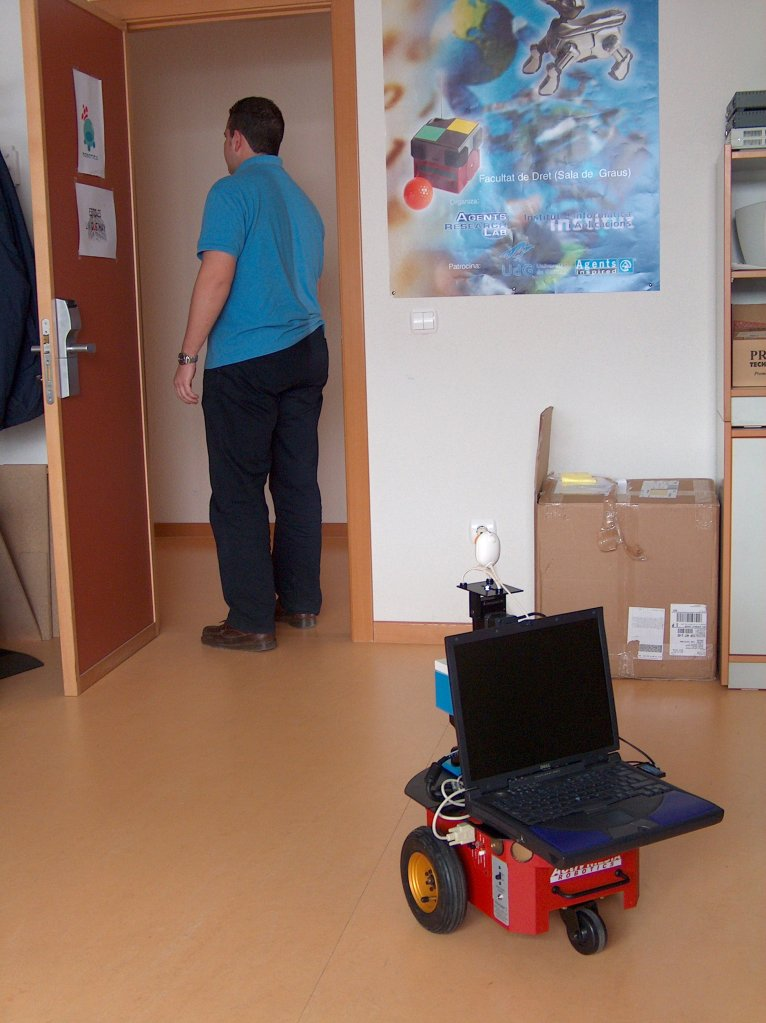
\includegraphics[width=3.5cm]{figs/moriles_sigue_persona.jpg}
 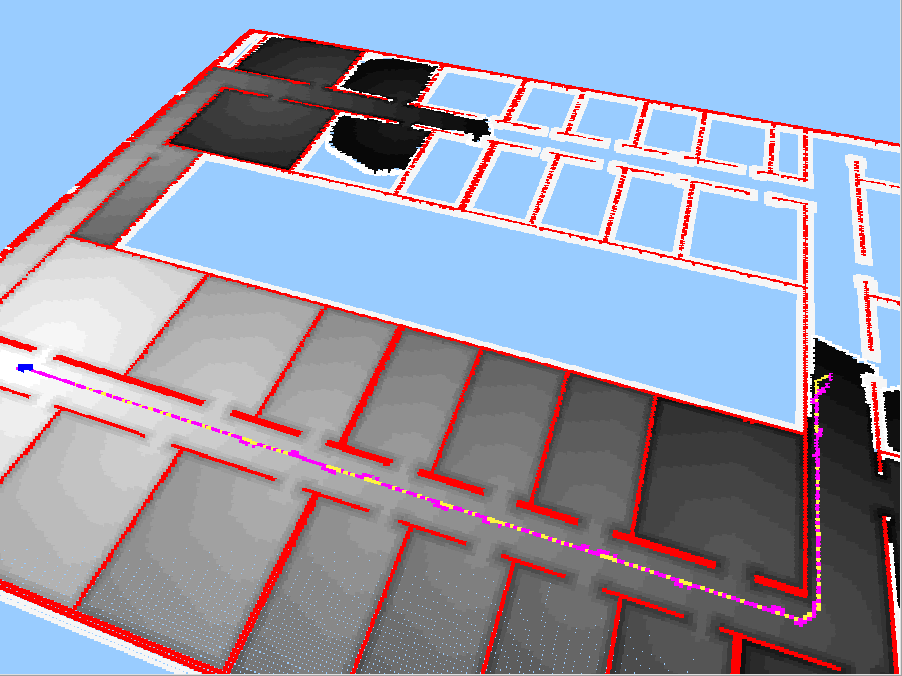
\includegraphics[width=4.5cm]{figs/gppNav.png}
\caption{Robot navigation using GPP and VFF algorithms.}
\label{fig:gppNav}
\end{figure}

When commanded to a position target our hybrid navigation method detects trap situations an then the robot slows down, the VFF algorithm is temporarily suspended and the GPP algotithm is then invoked to plan a new path based on the available information. GPP finds the optimal path to the goal at every point in the workspace (Figure \ref{fig:gppNav}). Currently we are working in kinect based navigation.

\subsection{Visual memory research}

The \texttt{VisualMemory} research component does a visual tracking of the various basic objects in the scene surrounding the robot to improve its navigation decisions. It detects new objects, tracks them updating their relative position to the robot and remove them from the memory once they have disappeared. An example of this visual memory contents is shown at Figure \ref{fig:memory} around a humanoid robot, built from several images of the camera on its mobile head.

\begin{figure}[h!]
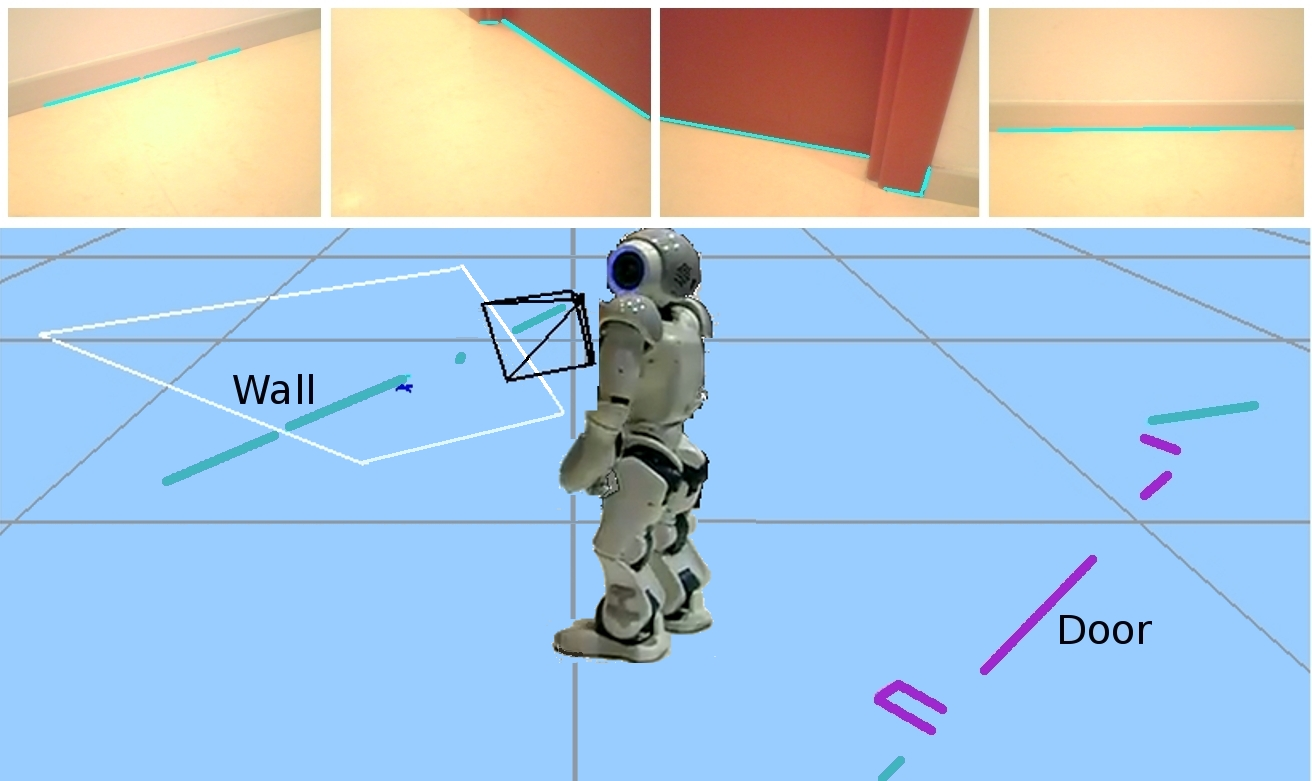
\includegraphics[width=8.5cm]{figs/experimentoReal.jpg}
\caption{Visual memory with 3D segments coming from four images of robot surroundings}
\label{fig:memory}
\end{figure}

The first stage of the system is a 2D analysis, in which segments in the current image are detected. These 2D segments are backprojected and put in 3D. In addition, each 3D visible object already stored in the visual memory is projected on the current image plane (using \texttt{Progeo}). The system refutes/corroborates such predicted segments comparing them with those extracted from current image. In case of matching the features of the stored 3D segment are updated taking into account the new observation. If a segment is identified in the current image but does not match any prediction, the system creates a new one in 3D. For predicted segments not really observed in current image their quality goes down and eventually will be removed from memory. Some post-processing is needed in visual memory to avoid duplicates due to noise in the images. This cleaning takes into account position, orientation and proximity of diferento segments to merge them, delete, etc.

\subsection{Evolutionary localization research}

Continuous and robust self-localization is at the moment one active research challenge in robotics. Using sensors such as cameras, laser or ultrasonic sensors, our robot must be able to calculate its own localization inside an environment. Once the robot knows its position, it can adapt its behavior depending on where it is located. However localization is a complex task on mobile robots, since they must face unknown situations, such as occlusions or dynamism of the environment. 

With Jderobot, we have designed and implemented an evolutionary localization algorithm, a meta-heuristic optimization algorithm that is inspired by the biological evolution. It manages a set of candidate positions that evolve over time using genetic operators, such as mutation or crossover. Several candidate solutions compete among each other in different positions. Thus, the evolutionary algorithm is able to handle several solutions at the same time, which is of great advantage when robots are located in symmetric environments.  

This research component has been tested both directly using as input images from \texttt{cameraServer} and using as input the visual memory built by the previous \texttt{VisualMemory} component. An specific ICE interface has been defined to this data communication between these two components.

\subsection{MonoSLAM research}

Monocular Simultaneous Localization And Mapping (MonoSLAM) is a type of localization first presented by Andrew J. Davison \cite{ref}. MonoSLAM is able to construct a point-based map of the environment with a single camera, and localizates the camera inside this environment in real time. We have developed our own MonoSLAM approach, based on Davison's work, obtaining images from real cameras or simulators. We first implemented the point-based approach designed by Andrew Davison and afterwards we have designed our own extensions that uses both relevant points and lines in the image flow.

This type of localization is more accurate than classical localization methods and is very useful when robot odometry is not available or is not reliable. On the other hand, it is not able to handle occlusions and needs a faster frame rate.

\subsection{Surveillance}

This application builds a surveillance distributed system that can be controlled using an smartphone. The system consists in some webcams and pc scattered around the house to watch over and detect any intruders or warning situations. Figure~\ref{fig:surveillance1} shows the Jderobot components that integrates this application. For each
webcam in the system there is an instance of \texttt{SrvRecorder} and
\texttt{CameraServer} components. The \texttt{SrvRecorder} component records the video streaming in the hard disk. The
\texttt{RecordingManager} component makes the configuration to
{SrvRecorder} components and decides when and how a recording is
made. The \texttt{CameraServer} component in Jderobot was expanded to provide the video streaming as
RTSP format or image format to analyze movement in the scene. The \texttt{Motion
  Detector} component makes a movement detection analysis of the
scene. If a movement is detected, it
sends a message to \texttt{Surveillance} component that has all the logic of
the security system. This component enables the \texttt{Recording Manager} component and sends messages to
start a recording when a movement is detected in the scene. Last, the
\texttt{SecurityApp} component executes in an Android device and
exchanges information with \texttt{RecordingManager} and
\texttt{CameraServer} to show recordings, alarms or video streaming live. It is also possible to see the recordings associated with the alarms. 

\begin{figure*}
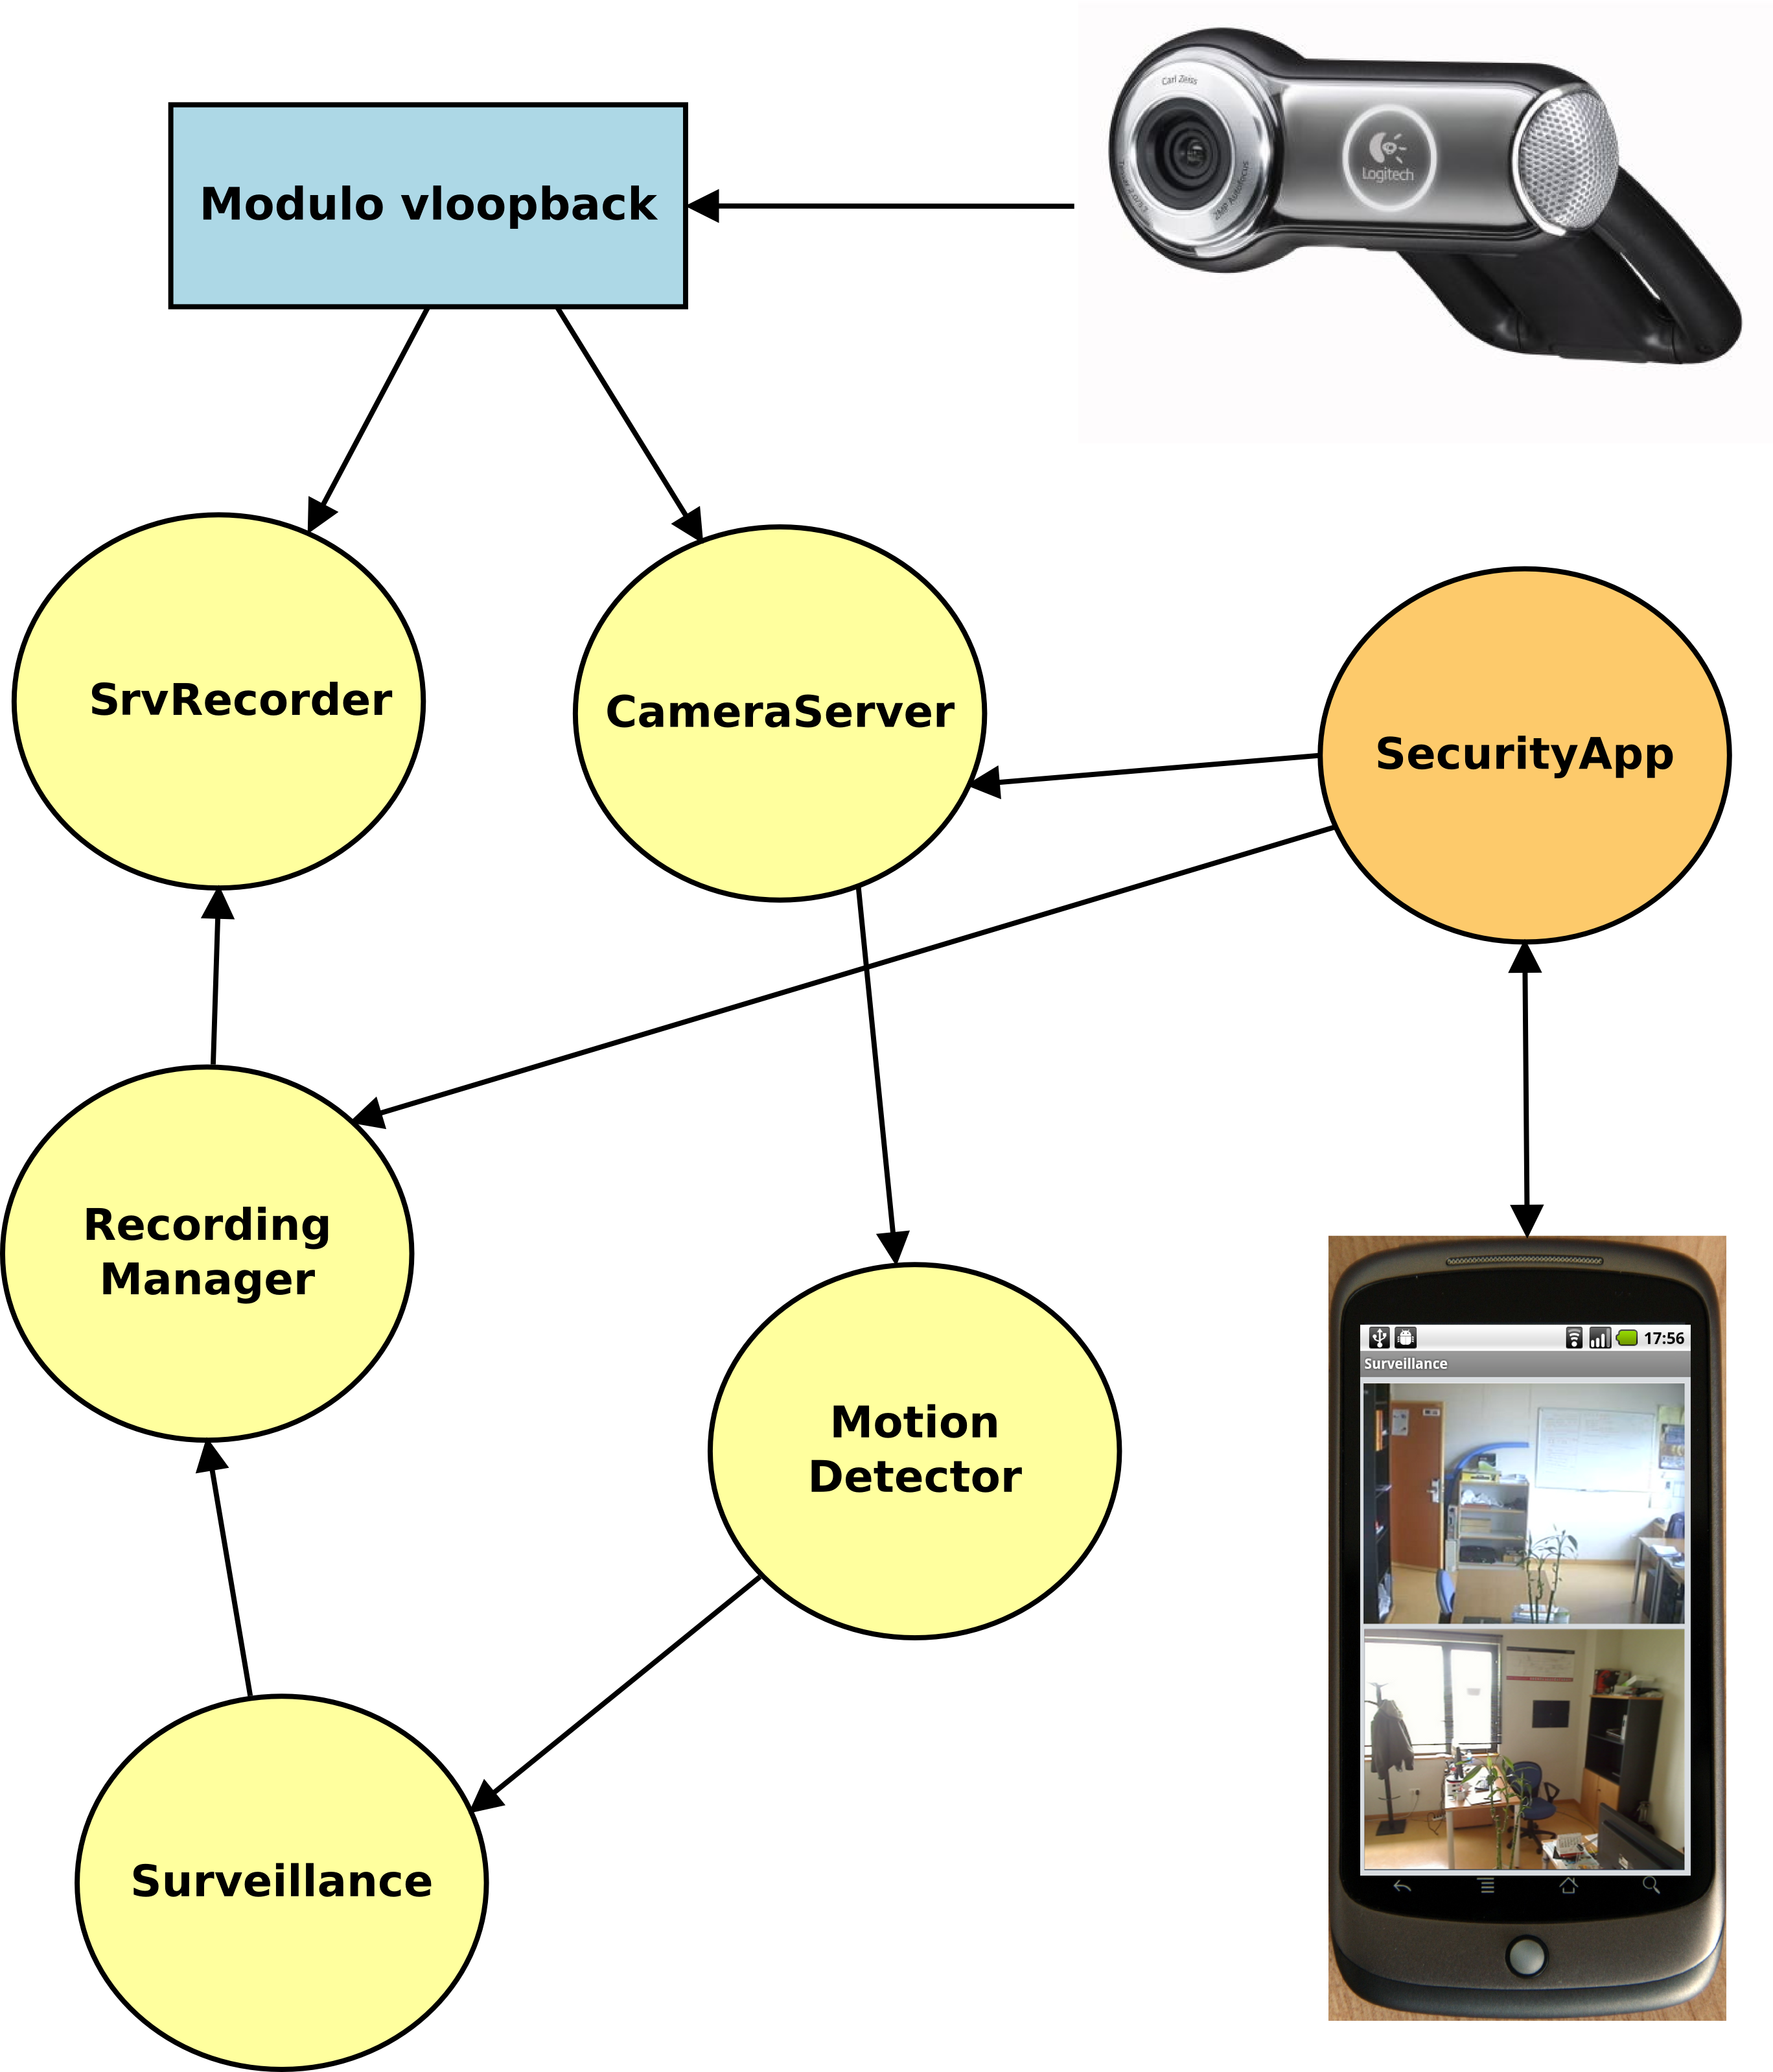
\includegraphics[width=6cm]{figs/surveillance-img1.png}
\caption{Jderobot components of Surveillance application}
\label{fig:surveillance1}
\end{figure*}

The mobile application is very simple thanks to the abstraction of the
jderobot components because you do not spend time in communication
protocols and other complex tasks. 
%You only have to worry about the functionality of the surveillance application. 
%For example, you can see in the figure~\ref{fig:surveillance2} the list of alarms that the \texttt{Recording Manager} component have stored. 
%The \texttt{CameraServer} component provides a video streaming live of the system webcams.

% You can see in the figure~\ref{fig:surveillance3} how it is possible show two video streamings live of the same room.

%% \begin{figure*}
%% 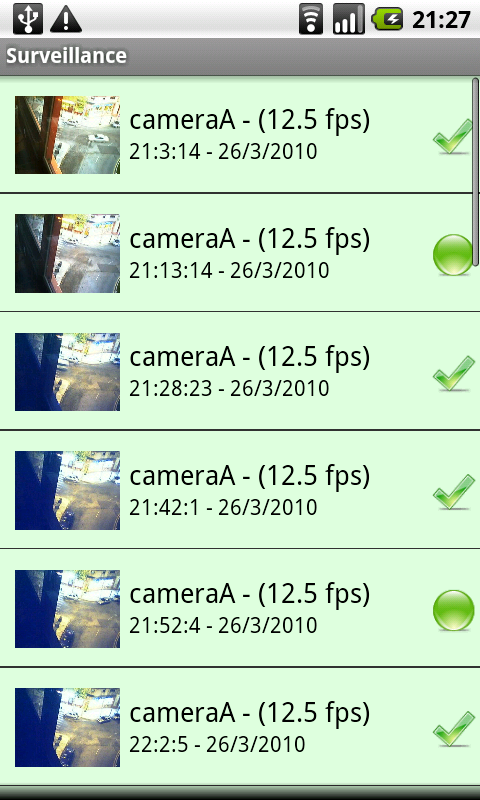
\includegraphics[width=6cm]{figs/surveillance-android.png}
%% \caption{Alarms list in the smartphone}
%% \label{fig:surveillance2}
%% \end{figure*}

%% \begin{figure*}
%% 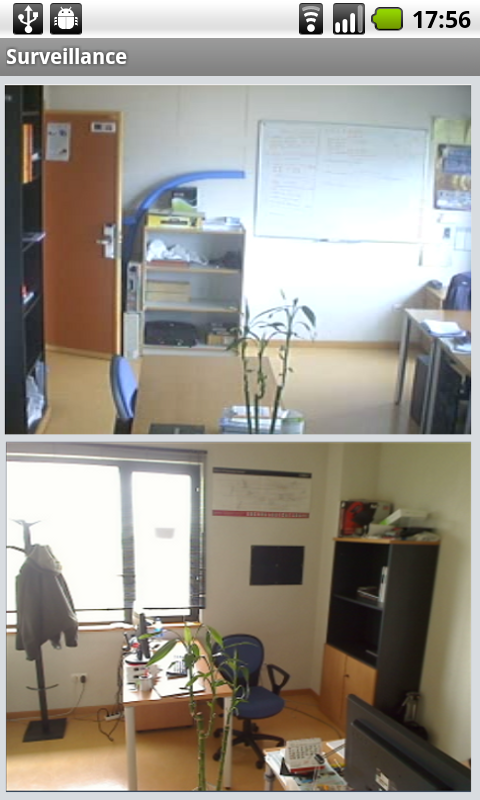
\includegraphics[width=6cm]{figs/surveillance-streaming2-recording.png}
%% \caption{Two video streaming of a room}
%% \label{fig:surveillance3}
%% \end{figure*}


\subsection{ElderCare}

Eldercare is a healthcare-oriented application for elderly people living alone. The system is able to autonomously detect falls using only conventional cameras. It uses one or several \texttt{CameraServer} components depending on which computers the cameras are attached to. An evolutive 3D tracking algorithm has been developed \cite{canas2011}.

Once a fall is detected the system automatically sends an alert to indicated medical personnel so that significantly reduces the waiting time for assistance. The system does not require any action by the patient, who does not need to wear any device over or any type of special garment. 
%It is a fully autonomous and non-intrusive system. Eldercare can handle all alarms on a mobile phone. 
When a fall is detected, it notifies the situation on a mobile phone and even allows to watch the scene in real time through streaming.

\begin{figure*}
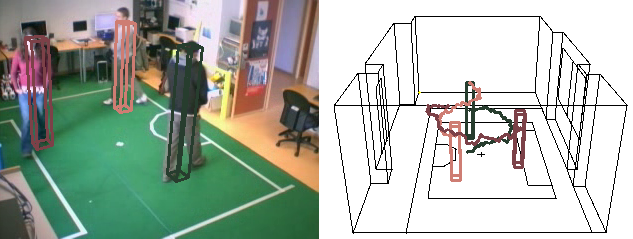
\includegraphics[width=8.5cm]{figs/eldercare.png}
\caption{Eldercare tracks 3D people position using cameras}
\label{fig:eldercare}
\end{figure*}

Currently we are doing research improving the 3D tracking algorithm to use Kinect devices. They are able to work as conventional cameras but have the main advantage of the on-board depth sensor. These devices work perfectly even without light, so the subject would be monitored in virtually any situation. Access to them is provided by \texttt{kinectServer} component.

\section{Jderobot as open-source project}

Jderobot project has a web page (jderobot.org) where the framework source code can be downloaded and its documentation accessed. The official manual is there in a MediaWiki. We prefer this web manual better than classic static documents, as the web manual update is agile and can be easily done by users themselves. We use a svn repository, trac for bug tracking, a blog and one mailing list for developers an users.

\subsection{Some history}

The Jderobot project started at 2002 in a PhD thesis, as the software implementation of a cognitive architecture to develop autonomous behaviors in robots \cite{canas02,canas05e}. It provided access to robot camera, encoders, sonar sensors and motors using sockets between some drivers and the (maybe remote) control application. The application was divided in \textit{schemas} that were implemented as concurrent threads in C language and organized as hierarchy. 

Its development was opened to a group of students. Several alternatives and expansions have been programmed since then \cite{canas07,canas07f}. A major revision was undergone in 2006 (jderobot-4.3). The design of schemas to be truly modular, they were programmed as dynamic libraries (plugins) which import and export symbols to other schemas. The XForms library for GUIs was replaced by GTK and OpenGL. In addition we started to use a common software repository and created a web page for the project. 

A second major revision was undergone in late 2010, leaving out the cognitive aspects and focusing in Jderobot simply as a software architecture for robot applications. The major design principles followed in this revision have been described in section \ref{sec:jderobot}. The current release, jderobot-5.0, is mainly based on this revision.

\subsection{Current release}
%current release and snapshot
Currently it has a total of 123.531 lines of source code, most of them
in C and C++ language. The SLOCCount tool can automatically identify
and measure a lot of languages of programming. Also, it includes
heuristics to detect type files and it estimates effort, time and
money about the development of the software.

\begin{verbatim}
SLOC    Directory        SLOC-by-Language 
60707   components (30)  cpp=32504,ansic=26370,
                         java=1355,xml=332,
                         sh=89,python=57
27509   interfaces (24)  cpp=27509
23620   share            xml=23620
11354   src_libs         cpp=9979,ansic=1375
338     debian           sh=338
3       scripts          sh=3
\end{verbatim}

Totals grouped by language
\begin{verbatim}
cpp:          69992 (56.66%)
ansic:        27745 (22.46%)
xml:          23952 (19.39%)
java:          1355 (1.10%)
sh:             430 (0.35%)
python:          57 (0.05%)
\end{verbatim}

\subsection{Study of the Jderobot community}
% jderobot community, who is using Jderobot
The Jderobot community includes members of the Robotics Group at Universidad Rey Juan Carlos, the Universidad de Málaga, Universidad Carlos III and Politécnico Colombiano Jaime Isaza Cadavid. The last two have already developed new driver components for their specific robots: a worm type robot and an all-terrain wheeled one, respectively.
% It is not very large

One user profile is a regular student of robotics courses at URJC. They don't have too much time to learn all the issues and power behind Jderobot, they just want to use it as soon as possible focusing on their robotic practices. To hide most of the complexity of robot programming and let the alumni to focus on the key aspects of robot control (not in GUI neither in communication middleware, etc) the \texttt{Introrob} component was developed. They just have to embbed their control algorithm in it. In a four month course (2 hours/week) they are able to use Jderobot and program a robot behavior with a Finite State Machine, a local navigation algorithm and a reactive visual control technique. 

%\texttt{apt-get install jderobot}
Some years ago only the Jderobot source code tarball was delivered to students and its installation was painful for them, with different library dependences, etc. The installation of the Jderobot teaching environment was greatly simplified when we developed Debian software packages for Gazebo and Jderobot.

A second user profile is a student from the URJC who uses Jderobot for their Final Degree Project, Master or PhD thesis. They usually become developers and extend the framework in some area. This way, the developer team has frequently changed along years. Until 2006 these students typically took a snapshot of Jderobot software at the beginning of their project, extended it and maybe debugged for its own purposes. This was really a bad practice as improvements to the framework were not easily shared among students. Since 2006, with the Jderobot modular design and a single repository this was solved, forcing the students to always run their code with the latest Jderobot release, and debug only the official release if needed.

\begin{figure}
  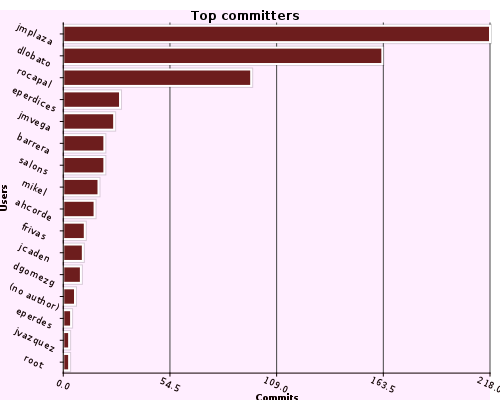
\includegraphics[width=7cm]{figs/svn_top-committers.png}
\caption{Top committers of Jderobot project}
\label{fig:svn-topcommiters}
\end{figure}

Some long term students have continuously contributed for several years, as can be seen at Figure \ref{fig:svn-topcommiters}. They have formed a stable developer core group of 4 or 5 people, all of them in a volunteer basis. In the last years we have opened the write access on Jderobot repository to relatively new users. Due to the large software size and the high rotation in the small developer team this has been very beneficial. The maintenance of the framework has already started to be more distributed.

\begin{figure}
  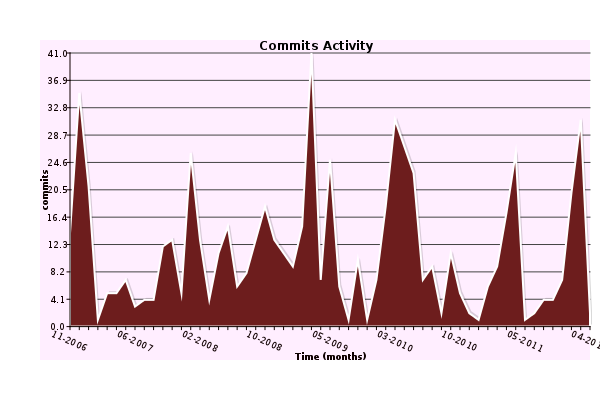
\includegraphics[width=7cm]{figs/svn_activity.png}
\caption{Activity of commits in the project}
\label{fig:svn-activity}
\end{figure}

Figure \ref{fig:svn-activity} shows the activity of software
improvement as number of commits in the official repository. The high
activity peaks are related with the release of a new Jderobot revision
and its debugging period.

All the graphics and metrics have been obtained by
CVSAnalY\footnote{http://projects.libresoft.es/projects/cvsanaly/wiki
}. CVSAnalY is a tool that extracts information out of
source code repository logs and stores it into a database. This FLOSS
project is developed by
GSyC/LibreSoft\footnote{http://www.libresoft.es}
 of Universidad Rey Juan Carlos.


\section{Conclusions}

%what have we presented in this paper
We have presented the Jderobot open-source framework for developing robotic applications and research. This is a long term effort with ten years of experience. It provides several drivers for accessing different sensors, robots and actuators like kinect, Nao humanoid, Pioneer robot, cameras, pantilt units, etc.. It also includes a powerful set of tools and libraries that speed up the creation of new robotic applications, like one for visual programming of hierarchical FSM, one for camera calibration, record of log files with sensor data and replay them, viewers and teleoperators, etc. Several successful applications and research components have been developed using the framework, they have been also presented as experimental validation of its usefulness.

%balance of design principles
The framework's main software architecture principle is the modular design of applications in concurrent components that interact among them through explicit standard interfaces. Each component is a software process, maybe with several threads, with a target. This modular design has proben to be easier to maintain and expand than previous monolithic and centralized releases of the framework. Only components relevant for a given application need to be installed and new functionality may appear as new components.

The standard interfaces have proben very advantageous for research. For instance, the same localization algorithm can be tested seemlessly with the real cameras, simulated ones, images from a video or from a log file as these image sources strictly follow the same interface. The portability between different robot platforms are also favored by standard interfaces. For example, experiments with the \texttt{VisualMemory} research component have been performed both in a wheeled Pioneer robot and a humanoid Nao robot without changing the source code, just providing the different robot geometry through configuration files, taking benefit of the same interfaces offered in both robot platforms.
% (camera, pose3Dencoders, pose3Dmotors and encoders)

The use of communication middleware like ICE provides Jderobot with multiplatform and multilanguage support, as components can be writen in C, C++, Java, Python, etc.. It also provides with distribution as the components can run in the same machine or different ones, even with different operating systems. For instance, a teleoperator has been presented with a component running in a smartphone interacting with the \texttt{NaoServer} in the Linux computer onboard the humanoid robot. Another advantage of using ICE is that we haven't taken much care of communications, focusing our efforts on robotics aspects of the components.

Iterative execution of components is recommended in Jderobot and it has proben good for reactive controllers, Bayesian estimators, localization algorithms or image processing applications. In addition, the programming of component GUI in a separate thread and its optional nature are also suggested, and they have shown to be advantageous as fully decouple the processing from the visualization, which can be switched on and off at run time at will without disturbing the robotic processing.

The intensive use of open-source tools and libraries has shown to be a good decision. They have allowed us to reach interesting functionality and results with a reduced set of developers, because we lie as much as possible on existing open-source community software like PCL, Gazebo, Opencv, OpenGL, GSL, etc. Software sharing speeds up and widen the project development. This belief has also motivated us to open the source code of Jderobot.

Two Jderobot's tools, the \texttt{recorder} and \texttt{replayer} components, are very useful in research. They allow, for instance, the fair comparison of different localization algorithms with exactly the same input data, those stored in the log file. A MonteCarlo localization algorithm has been so compared to our evolutive localization algorithm. In the same way, using our \texttt{CameraServer} from filed images our MonoSLAM algorithm have been tested with the same video images as the original Davison's MonoSLAM algorithm.

% more lessons 
We think Jderobot already has reached a good level of software reuse, but mainly for hardware abstraction layer. The same driver components and basic interfaces to access sensors and robots are used in different applications. This software reuse has not scaled yet to more complex robot functionality, maybe because the behavior abstraction is more slippery than traditional function invokation. We are working on this, focusing on reusable localization and local navigation components. The Jderobot tools have also been reused in different scenarios. For instance, the same calibration tool has been used to calibrate the cameras in \texttt{Eldercare} application, for the Nao humanoid camera or for the simulated cameras in Gazebo in the robotics course.

The developer team under Jderobot is small and with high rotation. One lesson learnt is that opening Jderobot development to several students, even new ones, is beneficial. Typical contribution is that of a new student becoming responsible of a single component, its development or updating. The modular design of Jderobot makes it possible. Another good decision has been to recommend our students that their applications should work always with the latest Jderobot release at the repository. This way bugs are solved in the official repository for everyone, everybody take benefit of their solution and there are no several co-existing branches at the same time.

The creation of Debian packages made easier the use of the platform in teaching, for newbie users that don't have time to fully learn the whole platforms in two weeks. In addition the specific IntroRob component hides some of the platform complexity, and so the students take shorter time to start using jderobot. 
The platform is just an instrument to learn robotics, not the goal.

%why not using ROS?
The use of communication middleware like ICE has allowed the programming of Jderobot components in smartphones easily interacting with other components in laptop or personal computers. This flexibility is a key difference between Jderobot and ROS. 

ROS set of drivers is larger than ours.

Tiene ROS un replay-recorder?.

%future lines
- Improved use of ICE advanced capabilities like Icestorm and Icebox.
- Wrappers to use drivers from other platforms wider than ours.

\begin{acknowledgements}
This work has been supported by the project S2009/DPI-1559, RoboCity2030-II, from the Comunidad de Madrid and by the project 10/02567 from the Spanish Ministry of Science and Innovation. Authors want also to thank the contribution to Jderobot project to all developers, in particular Alejandro Hernández and Maikel González.
\end{acknowledgements}

% BibTeX users please use one of
\bibliographystyle{spbasic}      % basic style, author-year citations
%\bibliographystyle{spmpsci}      % mathematics and physical sciences
%\bibliographystyle{spphys}       % APS-like style for physics
\bibliography{bibliografia}   % name your BibTeX data base


\end{document}


